\chapter{Realsierung des Projekts}
%**********************************************************************
% bild skizze Quelle; https://media.springernature.com/lw685/springer-static/image/chp%3A10.1007%2F978-3-658-34037-7_5/MediaObjects/507779_1_De_5_Fig2_HTML.png?as=webp
%*******************************************************************

\section{hardwaretechnische Umsetzung}
In diesem Abschnitt werden alle Maßnahemen für die hardwaretechnische Lösung aufgezeigt. Dabei wird die Funktionsweise erläutert und die technischen Spezifikationen dargelegt.
\subsection{Einsatz von Regalbediengeräten}
Die Gabelstapler werden durch Regalbediengeräten (RGB) ersetzt. Sie bewegen sich horizontal entlang von Schienen und vertikal zwischen den Regalebenen, wodurch sie Waren effizient transportieren können. 
Der technische Ablauf eines RGBs läuft in mehreren automatisierten Schritten ab, die durch ein Lagerverwaltungssystem (WMS), dargestellt in Kapitel ..., gesteuert werden. Für unsere Anordnung der Regale werden vier RGBs benötigt. Schienen und Führungselemente müssen dazu in den Zwischengängen installiert werden.

\subsection{Einsatz von Förderbänder}
Für den Weitertransport der Paletten innerhalb des Lagers werden Förderbänder eingesetzt, die eine zuverlässige und effiziente Verbindung zwischen Wareneingang, Hochregallager und Warenausgang ermöglichen. In unserem Projekt werden etwa 50 Meter Förderband benötigt, um alle relevanten Bereiche abzudecken. Dabei werden die Bänder direkt an die Regalbediengeräte und Warenschnittstellen angeschlossen, um einen nahtlosen Materialfluss sicherzustellen. Der Platz für die Installation ist gegeben.

\begin{figure}
	\centering
	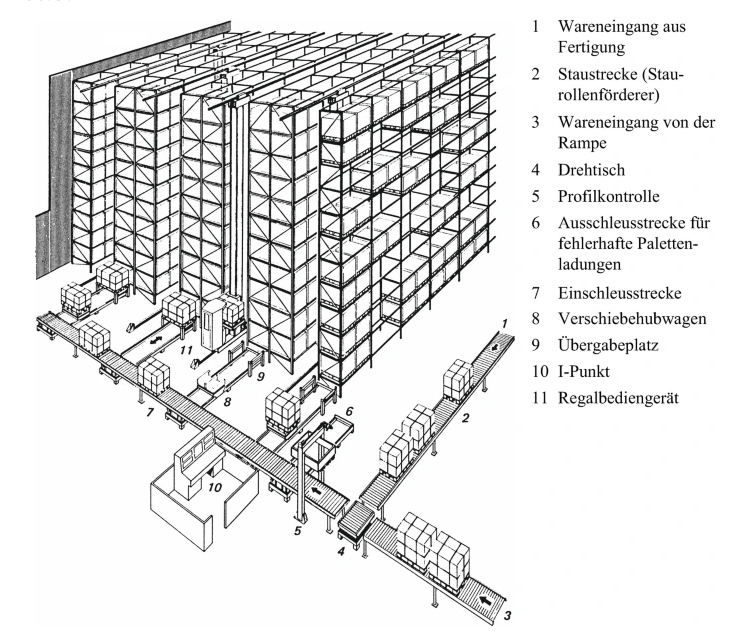
\includegraphics[width=0.7\linewidth]{images/skizze-Aufbau}
	\caption{schematische Darstellung mit der Implemtierung von RBGs und Föderbänderanlagen}
	\label{fig:skizze-aufbau}
\end{figure}

\section{softwaretechnische Lösung}
In diesem Abschnitt werden alle Maßnahemen für die softwaretechnische Lösung aufgezeigt. Hierbei besteht die herausforderung das Lagerverwaltungssystem mit den RGBs zu verknüpfen. Außerdem soll eine Verzahnung zwischen dem WMS und dem jetztigen genutzten ERP-System realisiert werden. Alle benötigte Sensorik und Aktorik sollen über IoT vernetzt werden.
\subsection{Implementierung des Lagerverwaltungssystem}
Das WMS wird in einer Cloud-basierten Lösung installiert und mit den Daten zu allen Lagerplätzen, Beständen und Aufträgen gefüttert. In einem initialen Schritt werden alle Lagerartikel in das System eingepflegt, sodass das WMS jederzeit den exakten Lagerbestand und die Positionen der Waren im Regal kennt. Es agiert als zentrale Plattform zur Verwaltung der Lagerprozesse, plant die Ein- und Auslagerungen, weist den Regalbediengeräten entsprechende Aufgaben zu und überwacht ihre Ausführung in Echtzeit.

\subsection{Verbindung mit ERP-System}
Um den gesamten Material- und Warenfluss effizient zu steuern, wird das WMS direkt mit dem ERP-System des Unternehmens verknüpft. Das ERP-System verwaltet die übergeordneten Geschäftsdaten wie Bestellungen, Lagerbestände und Produktionsanforderungen. Wenn beispielsweise eine neue Bestellung im ERP eingeht, übermittelt das System die Anforderungen an das WMS, welches daraufhin automatisch die Lageraufträge für die Regalbediengeräte erstellt.

Durch diese enge Verzahnung zwischen WMS und ERP können Warenbewegungen nahtlos in die Unternehmensprozesse integriert werden. Sobald ein Auftrag abgeschlossen ist, meldet das WMS die Informationen über die Bestandsänderungen zurück an das ERP-System, welches daraufhin die Bestands- und Finanzdaten aktualisiert.

\subsection{Vernetzung und IoT}
 Alle Geräte im Lager sind mit Sensoren ausgestattet und über das Internet der Dinge vernetzt. Diese Sensoren erfassen und übertragen in Echtzeit Daten wie Standort, Zustand und Energieverbrauch der Geräte. Das IoT ermöglicht es dem Unternehmen, den Zustand der Geräte kontinuierlich zu überwachen und Wartungen proaktiv durchzuführen, bevor es zu Störungen kommt.

\subsection{Künstliche Intelligenz zur Lageroptimierung}
Ist das System erstmal installiert, kann in naher Zukunft zur Optimierung der Logistik künstliche Intelligenz hinzugezogen werden. Künstliche Intelligenz kann die Abläufe im Lager optimieren, indem sie aus vergangenen Daten lernt und zukünftige Nachfrageprognosen erstellt. Maschinelles Lernen analysiert Bestellmuster und Lagerbewegungen, um die Lagerplatzierung von Artikeln zu optimieren und die Rüstzeiten zu reduzieren. Die Verwendung von künstlicher Intelligenz wird drigend geraten, um auch mit anderen Unternehmen in Zukunft wettbewerbsfähig zu bleiben.


\section{Ablauf}



	In der nachfolgende Auflistung wird der Ablauf der Warenbewegung durch RBGs im automatisierten Hochregallager beschrieben. Dabei werden die zentralen Schritte wie Auftragserteilung, Ein- und Auslagerung sowie die Kommunikation mit dem Lagerverwaltungssystem erläutert, die einen effizienten und präzisen Materialfluss sicherstellen.
\begin{enumerate}
	\item \textbf{Wareneingang und Anmeldung im ERP-System:}  
	Die eingehende Ware wird am Wareneingang überprüft und im \textbf{ERP-System} erfasst, welches die übergeordneten Geschäftsprozesse steuert. Das ERP-System übermittelt die relevanten Informationen, wie Artikelnummer, Menge und Lageranforderungen, an das \textbf{Warehouse Management System (WMS)}.
	
	\item \textbf{Lagerplatzzuweisung durch das WMS:}  
	Das \textbf{WMS} analysiert die Lagerkapazitäten und weist der Ware einen geeigneten Lagerplatz im Hochregal zu. Der Auftrag zur Einlagerung wird an das \textbf{Regalbediengerät (RBG)} weitergeleitet.
	
	\item \textbf{Einlagerung durch das RBG:}  
	Das \textbf{RBG} empfängt den Einlagerungsauftrag und fährt entlang der horizontalen und vertikalen Schienen zur zugewiesenen Regalposition. Mithilfe von Sensoren und Kamerasystemen überprüft das RBG die exakte Position und schiebt die Palette präzise in das zugewiesene Lagerfach. Nach Abschluss der Einlagerung sendet das RBG eine Rückmeldung an das WMS, das den Lagerbestand aktualisiert.
	
	\item \textbf{Lagerverwaltung und Zwischenlagerung:}  
	Während die Waren im Hochregal lagern, überwacht das \textbf{WMS} kontinuierlich die Bestände und meldet bei Bedarf Daten an das \textbf{ERP-System} zurück, z. B. zur Produktionsplanung oder Nachbestellung. Eine regelmäßige Bestandspflege erfolgt automatisch durch Sensoren und Rückmeldungen der RBGs.
	
	\item \textbf{Auftragserteilung für den Warenausgang:}  
	Bei Bedarf (z. B. durch Kundenbestellungen oder Produktionsanforderungen) erstellt das \textbf{ERP-System} einen Auslagerungsauftrag. Das ERP-System übermittelt diesen Auftrag an das \textbf{WMS}, das die optimalen Warenplätze für den Abruf ermittelt.
	
	\item \textbf{Auslagerung durch das RBG:}  
	Das \textbf{WMS} weist dem \textbf{RBG} die zu entnehmende Ware zu, inklusive der genauen Regalposition. Das RBG fährt zur angegebenen Position, entnimmt die Ware präzise und transportiert sie zur Übergabestation.
	
	\item \textbf{Weitertransport durch Förderbänder:}  
	Die Ware wird von der Übergabestation des RBGs automatisch auf das \textbf{Förderbandsystem} übergeben. Das Förderband transportiert die Paletten zum Warenausgang oder einem definierten Übergabepunkt für den Versand.
	
	\item \textbf{Abschluss im ERP-System:}  
	Sobald die Ware den Warenausgang erreicht, wird dies automatisch an das \textbf{ERP-System} zurückgemeldet. Das ERP-System aktualisiert den Bestand, erstellt die Versanddokumente und schließt den Auftrag ab.
	
\end{enumerate}